\documentclass[1p]{elsarticle_modified}
%\bibliographystyle{elsarticle-num}

%\usepackage[colorlinks]{hyperref}
%\usepackage{abbrmath_seonhwa} %\Abb, \Ascr, \Acal ,\Abf, \Afrak
\usepackage{amsfonts}
\usepackage{amssymb}
\usepackage{amsmath}
\usepackage{amsthm}
\usepackage{scalefnt}
\usepackage{amsbsy}
\usepackage{kotex}
\usepackage{caption}
\usepackage{subfig}
\usepackage{color}
\usepackage{graphicx}
\usepackage{xcolor} %% white, black, red, green, blue, cyan, magenta, yellow
\usepackage{float}
\usepackage{setspace}
\usepackage{hyperref}

\usepackage{tikz}
\usetikzlibrary{arrows}

\usepackage{multirow}
\usepackage{array} % fixed length table
\usepackage{hhline}

%%%%%%%%%%%%%%%%%%%%%
\makeatletter
\renewcommand*\env@matrix[1][\arraystretch]{%
	\edef\arraystretch{#1}%
	\hskip -\arraycolsep
	\let\@ifnextchar\new@ifnextchar
	\array{*\c@MaxMatrixCols c}}
\makeatother %https://tex.stackexchange.com/questions/14071/how-can-i-increase-the-line-spacing-in-a-matrix
%%%%%%%%%%%%%%%

\usepackage[normalem]{ulem}

\newcommand{\msout}[1]{\ifmmode\text{\sout{\ensuremath{#1}}}\else\sout{#1}\fi}
%SOURCE: \msout is \stkout macro in https://tex.stackexchange.com/questions/20609/strikeout-in-math-mode

\newcommand{\cancel}[1]{
	\ifmmode
	{\color{red}\msout{#1}}
	\else
	{\color{red}\sout{#1}}
	\fi
}

\newcommand{\add}[1]{
	{\color{blue}\uwave{#1}}
}

\newcommand{\replace}[2]{
	\ifmmode
	{\color{red}\msout{#1}}{\color{blue}\uwave{#2}}
	\else
	{\color{red}\sout{#1}}{\color{blue}\uwave{#2}}
	\fi
}

\newcommand{\Sol}{\mathcal{S}} %segment
\newcommand{\D}{D} %diagram
\newcommand{\A}{\mathcal{A}} %arc


%%%%%%%%%%%%%%%%%%%%%%%%%%%%%5 test

\def\sl{\operatorname{\textup{SL}}(2,\Cbb)}
\def\psl{\operatorname{\textup{PSL}}(2,\Cbb)}
\def\quan{\mkern 1mu \triangleright \mkern 1mu}

\theoremstyle{definition}
\newtheorem{thm}{Theorem}[section]
\newtheorem{prop}[thm]{Proposition}
\newtheorem{lem}[thm]{Lemma}
\newtheorem{ques}[thm]{Question}
\newtheorem{cor}[thm]{Corollary}
\newtheorem{defn}[thm]{Definition}
\newtheorem{exam}[thm]{Example}
\newtheorem{rmk}[thm]{Remark}
\newtheorem{alg}[thm]{Algorithm}

\newcommand{\I}{\sqrt{-1}}
\begin{document}

%\begin{frontmatter}
%
%\title{Boundary parabolic representations of knots up to 8 crossings}
%
%%% Group authors per affiliation:
%\author{Yunhi Cho} 
%\address{Department of Mathematics, University of Seoul, Seoul, Korea}
%\ead{yhcho@uos.ac.kr}
%
%
%\author{Seonhwa Kim} %\fnref{s_kim}}
%\address{Center for Geometry and Physics, Institute for Basic Science, Pohang, 37673, Korea}
%\ead{ryeona17@ibs.re.kr}
%
%\author{Hyuk Kim}
%\address{Department of Mathematical Sciences, Seoul National University, Seoul 08826, Korea}
%\ead{hyukkim@snu.ac.kr}
%
%\author{Seokbeom Yoon}
%\address{Department of Mathematical Sciences, Seoul National University, Seoul, 08826,  Korea}
%\ead{sbyoon15@snu.ac.kr}
%
%\begin{abstract}
%We find all boundary parabolic representation of knots up to 8 crossings.
%
%\end{abstract}
%\begin{keyword}
%    \MSC[2010] 57M25 
%\end{keyword}
%
%\end{frontmatter}

%\linenumbers
%\tableofcontents
%
\newcommand\colored[1]{\textcolor{white}{\rule[-0.35ex]{0.8em}{1.4ex}}\kern-0.8em\color{red} #1}%
%\newcommand\colored[1]{\textcolor{white}{ #1}\kern-2.17ex	\textcolor{white}{ #1}\kern-1.81ex	\textcolor{white}{ #1}\kern-2.15ex\color{red}#1	}

{\Large $\underline{12a_{0330}~(K12a_{0330})}$}

\setlength{\tabcolsep}{10pt}
\renewcommand{\arraystretch}{1.6}
\vspace{1cm}\begin{tabular}{m{100pt}>{\centering\arraybackslash}m{274pt}}
\multirow{5}{120pt}{
	\centering
	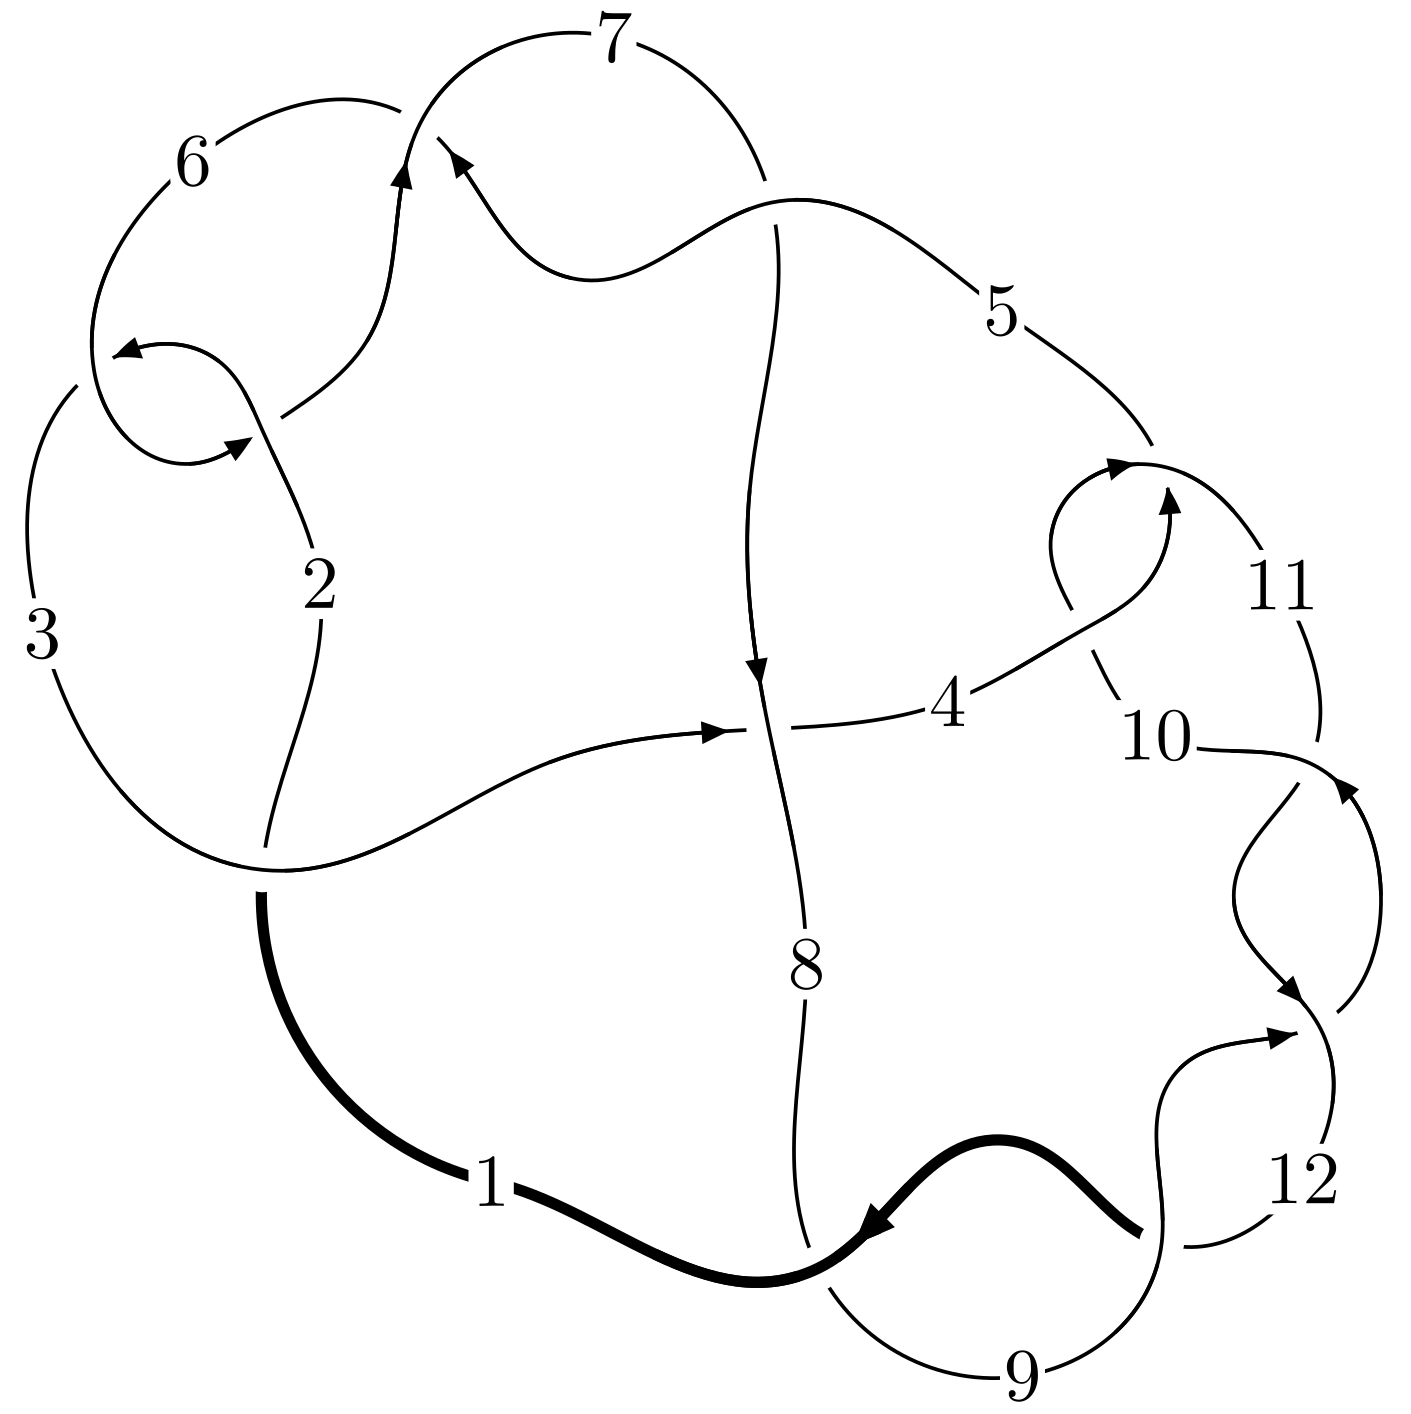
\includegraphics[width=112pt]{../../../GIT/diagram.site/Diagrams/png/1131_12a_0330.png}\\
\ \ \ A knot diagram\footnotemark}&
\allowdisplaybreaks
\textbf{Linearized knot diagam} \\
\cline{2-2}
 &
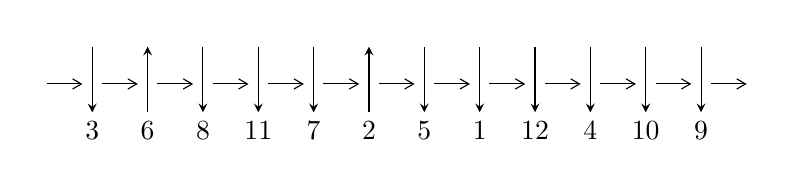
\begin{tikzpicture}[x=20pt, y=17pt]
	% nodes
	\node (C0) at (0, 0) {};
	\node (C1) at (1, 0) {};
	\node (C1U) at (1, +1) {};
	\node (C1D) at (1, -1) {3};

	\node (C2) at (2, 0) {};
	\node (C2U) at (2, +1) {};
	\node (C2D) at (2, -1) {6};

	\node (C3) at (3, 0) {};
	\node (C3U) at (3, +1) {};
	\node (C3D) at (3, -1) {8};

	\node (C4) at (4, 0) {};
	\node (C4U) at (4, +1) {};
	\node (C4D) at (4, -1) {11};

	\node (C5) at (5, 0) {};
	\node (C5U) at (5, +1) {};
	\node (C5D) at (5, -1) {7};

	\node (C6) at (6, 0) {};
	\node (C6U) at (6, +1) {};
	\node (C6D) at (6, -1) {2};

	\node (C7) at (7, 0) {};
	\node (C7U) at (7, +1) {};
	\node (C7D) at (7, -1) {5};

	\node (C8) at (8, 0) {};
	\node (C8U) at (8, +1) {};
	\node (C8D) at (8, -1) {1};

	\node (C9) at (9, 0) {};
	\node (C9U) at (9, +1) {};
	\node (C9D) at (9, -1) {12};

	\node (C10) at (10, 0) {};
	\node (C10U) at (10, +1) {};
	\node (C10D) at (10, -1) {4};

	\node (C11) at (11, 0) {};
	\node (C11U) at (11, +1) {};
	\node (C11D) at (11, -1) {10};

	\node (C12) at (12, 0) {};
	\node (C12U) at (12, +1) {};
	\node (C12D) at (12, -1) {9};
	\node (C13) at (13, 0) {};

	% arrows
	\draw[->,>={angle 60}]
	(C0) edge (C1) (C1) edge (C2) (C2) edge (C3) (C3) edge (C4) (C4) edge (C5) (C5) edge (C6) (C6) edge (C7) (C7) edge (C8) (C8) edge (C9) (C9) edge (C10) (C10) edge (C11) (C11) edge (C12) (C12) edge (C13) ;	\draw[->,>=stealth]
	(C1U) edge (C1D) (C2D) edge (C2U) (C3U) edge (C3D) (C4U) edge (C4D) (C5U) edge (C5D) (C6D) edge (C6U) (C7U) edge (C7D) (C8U) edge (C8D) (C9U) edge (C9D) (C10U) edge (C10D) (C11U) edge (C11D) (C12U) edge (C12D) ;
	\end{tikzpicture} \\
\hhline{~~} \\& 
\textbf{Solving Sequence} \\ \cline{2-2} 
 &
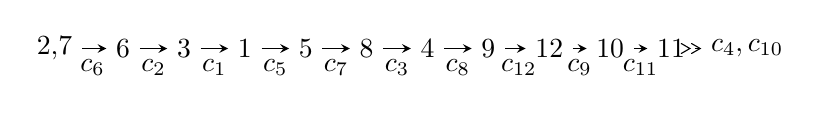
\begin{tikzpicture}[x=22pt, y=7pt]
	% node
	\node (A0) at (-1/8, 0) {2,7};
	\node (A1) at (1, 0) {6};
	\node (A2) at (2, 0) {3};
	\node (A3) at (3, 0) {1};
	\node (A4) at (4, 0) {5};
	\node (A5) at (5, 0) {8};
	\node (A6) at (6, 0) {4};
	\node (A7) at (7, 0) {9};
	\node (A8) at (8, 0) {12};
	\node (A9) at (9, 0) {10};
	\node (A10) at (10, 0) {11};
	\node (C1) at (1/2, -1) {$c_{6}$};
	\node (C2) at (3/2, -1) {$c_{2}$};
	\node (C3) at (5/2, -1) {$c_{1}$};
	\node (C4) at (7/2, -1) {$c_{5}$};
	\node (C5) at (9/2, -1) {$c_{7}$};
	\node (C6) at (11/2, -1) {$c_{3}$};
	\node (C7) at (13/2, -1) {$c_{8}$};
	\node (C8) at (15/2, -1) {$c_{12}$};
	\node (C9) at (17/2, -1) {$c_{9}$};
	\node (C10) at (19/2, -1) {$c_{11}$};
	\node (A11) at (45/4, 0) {$c_{4},c_{10}$};

	% edge
	\draw[->,>=stealth]	
	(A0) edge (A1) (A1) edge (A2) (A2) edge (A3) (A3) edge (A4) (A4) edge (A5) (A5) edge (A6) (A6) edge (A7) (A7) edge (A8) (A8) edge (A9) (A9) edge (A10) ;
	\draw[->>,>={angle 60}]	
	(A10) edge (A11);
\end{tikzpicture} \\ 

\end{tabular} \\

\footnotetext{
The image of knot diagram is generated by the software ``\textbf{Draw programme}" developed by Andrew Bartholomew(\url{http://www.layer8.co.uk/maths/draw/index.htm\#Running-draw}), where we modified some parts for our purpose(\url{https://github.com/CATsTAILs/LinksPainter}).
}\phantom \\ \newline 
\centering \textbf{Ideals for irreducible components\footnotemark of $X_{\text{par}}$} 
 
\begin{align*}
I^u_{1}&=\langle 
u^{47}+u^{46}+\cdots+2 u-1\rangle \\
\\
\end{align*}
\raggedright * 1 irreducible components of $\dim_{\mathbb{C}}=0$, with total 47 representations.\\
\footnotetext{All coefficients of polynomials are rational numbers. But the coefficients are sometimes approximated in decimal forms when there is not enough margin.}
\newpage
\renewcommand{\arraystretch}{1}
\centering \section*{I. $I^u_{1}= \langle u^{47}+u^{46}+\cdots+2 u-1 \rangle$}
\flushleft \textbf{(i) Arc colorings}\\
\begin{tabular}{m{7pt} m{180pt} m{7pt} m{180pt} }
\flushright $a_{2}=$&$\begin{pmatrix}0\\u\end{pmatrix}$ \\
\flushright $a_{7}=$&$\begin{pmatrix}1\\0\end{pmatrix}$ \\
\flushright $a_{6}=$&$\begin{pmatrix}1\\u^2\end{pmatrix}$ \\
\flushright $a_{3}=$&$\begin{pmatrix}u\\u^3+u\end{pmatrix}$ \\
\flushright $a_{1}=$&$\begin{pmatrix}u^3\\u^5+u^3+u\end{pmatrix}$ \\
\flushright $a_{5}=$&$\begin{pmatrix}u^2+1\\u^2\end{pmatrix}$ \\
\flushright $a_{8}=$&$\begin{pmatrix}u^4+u^2+1\\u^4\end{pmatrix}$ \\
\flushright $a_{4}=$&$\begin{pmatrix}- u^{11}-2 u^9-4 u^7-4 u^5-3 u^3\\- u^{11}- u^9-2 u^7- u^5+u^3+u\end{pmatrix}$ \\
\flushright $a_{9}=$&$\begin{pmatrix}u^{12}+u^{10}+3 u^8+2 u^6+2 u^4+u^2+1\\u^{14}+2 u^{12}+5 u^{10}+6 u^8+6 u^6+4 u^4+u^2\end{pmatrix}$ \\
\flushright $a_{12}=$&$\begin{pmatrix}u^{21}+2 u^{19}+\cdots+4 u^3+u\\u^{23}+3 u^{21}+\cdots+2 u^3+u\end{pmatrix}$ \\
\flushright $a_{10}=$&$\begin{pmatrix}u^{30}+3 u^{28}+\cdots+2 u^2+1\\u^{32}+4 u^{30}+\cdots+8 u^4+2 u^2\end{pmatrix}$ \\
\flushright $a_{11}=$&$\begin{pmatrix}u^{39}+4 u^{37}+\cdots+8 u^3+2 u\\u^{41}+5 u^{39}+\cdots+4 u^3+u\end{pmatrix}$\\&\end{tabular}
\flushleft \textbf{(ii) Obstruction class $= -1$}\\~\\
\flushleft \textbf{(iii) Cusp Shapes $= -4 u^{46}-20 u^{44}+\cdots+20 u-14$}\\~\\
\newpage\renewcommand{\arraystretch}{1}
\flushleft \textbf{(iv) u-Polynomials at the component}\newline \\
\begin{tabular}{m{50pt}|m{274pt}}
Crossings & \hspace{64pt}u-Polynomials at each crossing \\
\hline $$\begin{aligned}c_{1},c_{5},c_{7}\end{aligned}$$&$\begin{aligned}
&u^{47}+11 u^{46}+\cdots+16 u^2-1
\end{aligned}$\\
\hline $$\begin{aligned}c_{2},c_{6}\end{aligned}$$&$\begin{aligned}
&u^{47}- u^{46}+\cdots+2 u+1
\end{aligned}$\\
\hline $$\begin{aligned}c_{3}\end{aligned}$$&$\begin{aligned}
&u^{47}- u^{46}+\cdots-6060 u+3361
\end{aligned}$\\
\hline $$\begin{aligned}c_{4},c_{10}\end{aligned}$$&$\begin{aligned}
&u^{47}- u^{46}+\cdots+2 u+1
\end{aligned}$\\
\hline $$\begin{aligned}c_{8},c_{9},c_{11}\\c_{12}\end{aligned}$$&$\begin{aligned}
&u^{47}+9 u^{46}+\cdots+4 u^2+1
\end{aligned}$\\
\hline
\end{tabular}\\~\\
\newpage\renewcommand{\arraystretch}{1}
\flushleft \textbf{(v) Riley Polynomials at the component}\newline \\
\begin{tabular}{m{50pt}|m{274pt}}
Crossings & \hspace{64pt}Riley Polynomials at each crossing \\
\hline $$\begin{aligned}c_{1},c_{5},c_{7}\end{aligned}$$&$\begin{aligned}
&y^{47}+51 y^{46}+\cdots+32 y-1
\end{aligned}$\\
\hline $$\begin{aligned}c_{2},c_{6}\end{aligned}$$&$\begin{aligned}
&y^{47}+11 y^{46}+\cdots+16 y^2-1
\end{aligned}$\\
\hline $$\begin{aligned}c_{3}\end{aligned}$$&$\begin{aligned}
&y^{47}+31 y^{46}+\cdots+5775512 y-11296321
\end{aligned}$\\
\hline $$\begin{aligned}c_{4},c_{10}\end{aligned}$$&$\begin{aligned}
&y^{47}-9 y^{46}+\cdots-4 y^2-1
\end{aligned}$\\
\hline $$\begin{aligned}c_{8},c_{9},c_{11}\\c_{12}\end{aligned}$$&$\begin{aligned}
&y^{47}+59 y^{46}+\cdots-8 y-1
\end{aligned}$\\
\hline
\end{tabular}\\~\\
\newpage\flushleft \textbf{(vi) Complex Volumes and Cusp Shapes}
$$\begin{array}{c|c|c}  
\text{Solutions to }I^u_{1}& \I (\text{vol} + \sqrt{-1}CS) & \text{Cusp shape}\\
 \hline 
\begin{aligned}
u &= \phantom{-}0.382879 + 0.913206 I\end{aligned}
 & -0.08570 + 6.28148 I & -8.16298 - 10.47100 I \\ \hline\begin{aligned}
u &= \phantom{-}0.382879 - 0.913206 I\end{aligned}
 & -0.08570 - 6.28148 I & -8.16298 + 10.47100 I \\ \hline\begin{aligned}
u &= \phantom{-}0.008475 + 0.965301 I\end{aligned}
 & \phantom{-}6.38651 - 3.25280 I & -8.46380 + 2.37401 I \\ \hline\begin{aligned}
u &= \phantom{-}0.008475 - 0.965301 I\end{aligned}
 & \phantom{-}6.38651 + 3.25280 I & -8.46380 - 2.37401 I \\ \hline\begin{aligned}
u &= -0.413985 + 0.853429 I\end{aligned}
 & \phantom{-}0.89586 - 2.03383 I & -4.23793 + 3.81818 I \\ \hline\begin{aligned}
u &= -0.413985 - 0.853429 I\end{aligned}
 & \phantom{-}0.89586 + 2.03383 I & -4.23793 - 3.81818 I \\ \hline\begin{aligned}
u &= -0.456667 + 0.956333 I\end{aligned}
 & \phantom{-}9.00501 - 2.08590 I & -4.31423 + 3.31096 I \\ \hline\begin{aligned}
u &= -0.456667 - 0.956333 I\end{aligned}
 & \phantom{-}9.00501 + 2.08590 I & -4.31423 - 3.31096 I \\ \hline\begin{aligned}
u &= \phantom{-}0.446885 + 0.962913 I\end{aligned}
 & \phantom{-}8.85349 + 8.66849 I & -4.72563 - 8.03831 I \\ \hline\begin{aligned}
u &= \phantom{-}0.446885 - 0.962913 I\end{aligned}
 & \phantom{-}8.85349 - 8.66849 I & -4.72563 + 8.03831 I \\ \hline\begin{aligned}
u &= \phantom{-}0.276872 + 0.873166 I\end{aligned}
 & -3.20238 + 2.30452 I & -16.3116 - 5.9470 I \\ \hline\begin{aligned}
u &= \phantom{-}0.276872 - 0.873166 I\end{aligned}
 & -3.20238 - 2.30452 I & -16.3116 + 5.9470 I \\ \hline\begin{aligned}
u &= \phantom{-}0.112869 + 0.850703 I\end{aligned}
 & -1.52782 - 1.56803 I & -12.46880 + 3.57703 I \\ \hline\begin{aligned}
u &= \phantom{-}0.112869 - 0.850703 I\end{aligned}
 & -1.52782 + 1.56803 I & -12.46880 - 3.57703 I \\ \hline\begin{aligned}
u &= -0.820103 + 0.872946 I\end{aligned}
 & \phantom{-}3.33252 - 0.63798 I & -8.00000 - 1.61055 I \\ \hline\begin{aligned}
u &= -0.820103 - 0.872946 I\end{aligned}
 & \phantom{-}3.33252 + 0.63798 I & -8.00000 + 1.61055 I \\ \hline\begin{aligned}
u &= -0.866477 + 0.852451 I\end{aligned}
 & \phantom{-}7.76984 + 3.47355 I & -2.51866 - 3.95961 I \\ \hline\begin{aligned}
u &= -0.866477 - 0.852451 I\end{aligned}
 & \phantom{-}7.76984 - 3.47355 I & -2.51866 + 3.95961 I \\ \hline\begin{aligned}
u &= -0.808162 + 0.922528 I\end{aligned}
 & \phantom{-}3.18030 - 5.45437 I & -8.00000 + 6.66748 I \\ \hline\begin{aligned}
u &= -0.808162 - 0.922528 I\end{aligned}
 & \phantom{-}3.18030 + 5.45437 I & -8.00000 - 6.66748 I \\ \hline\begin{aligned}
u &= -0.680659 + 0.361501 I\end{aligned}
 & \phantom{-}10.90210 - 2.07362 I & \phantom{-}0.04088 + 2.30391 I \\ \hline\begin{aligned}
u &= -0.680659 - 0.361501 I\end{aligned}
 & \phantom{-}10.90210 + 2.07362 I & \phantom{-}0.04088 - 2.30391 I \\ \hline\begin{aligned}
u &= \phantom{-}0.867742 + 0.871991 I\end{aligned}
 & \phantom{-}8.77828 + 1.40174 I & \phantom{-0.000000 } 0. - 2.33106 I \\ \hline\begin{aligned}
u &= \phantom{-}0.867742 - 0.871991 I\end{aligned}
 & \phantom{-}8.77828 - 1.40174 I & \phantom{-0.000000 -}0. + 2.33106 I \\ \hline\begin{aligned}
u &= \phantom{-}0.835618 + 0.904887 I\end{aligned}
 & \phantom{-}6.11156 + 3.11267 I & \phantom{-0.000000 } 0. - 2.66928 I \\ \hline\begin{aligned}
u &= \phantom{-}0.835618 - 0.904887 I\end{aligned}
 & \phantom{-}6.11156 - 3.11267 I & \phantom{-0.000000 -}0. + 2.66928 I \\ \hline\begin{aligned}
u &= \phantom{-}0.681301 + 0.344571 I\end{aligned}
 & \phantom{-}10.82780 - 4.54766 I & -0.10220 + 2.48977 I \\ \hline\begin{aligned}
u &= \phantom{-}0.681301 - 0.344571 I\end{aligned}
 & \phantom{-}10.82780 + 4.54766 I & -0.10220 - 2.48977 I \\ \hline\begin{aligned}
u &= -0.284938 + 0.707717 I\end{aligned}
 & -0.343803 - 1.199580 I & -4.23003 + 5.53729 I \\ \hline\begin{aligned}
u &= -0.284938 - 0.707717 I\end{aligned}
 & -0.343803 + 1.199580 I & -4.23003 - 5.53729 I\\
 \hline 
 \end{array}$$\newpage$$\begin{array}{c|c|c}  
\text{Solutions to }I^u_{1}& \I (\text{vol} + \sqrt{-1}CS) & \text{Cusp shape}\\
 \hline 
\begin{aligned}
u &= -0.900013 + 0.851367 I\end{aligned}
 & \phantom{-}17.6045 + 6.0118 I & \phantom{-0.000000 } 0. - 2.53476 I \\ \hline\begin{aligned}
u &= -0.900013 - 0.851367 I\end{aligned}
 & \phantom{-}17.6045 - 6.0118 I & \phantom{-0.000000 -}0. + 2.53476 I \\ \hline\begin{aligned}
u &= \phantom{-}0.900037 + 0.855771 I\end{aligned}
 & \phantom{-}17.8006 + 0.6918 I & \phantom{-0.000000 } 0. - 2.07521 I \\ \hline\begin{aligned}
u &= \phantom{-}0.900037 - 0.855771 I\end{aligned}
 & \phantom{-}17.8006 - 0.6918 I & \phantom{-0.000000 -}0. + 2.07521 I \\ \hline\begin{aligned}
u &= \phantom{-}0.838574 + 0.946010 I\end{aligned}
 & \phantom{-}8.54527 + 4.93007 I & \phantom{-0.000000 } 0 \\ \hline\begin{aligned}
u &= \phantom{-}0.838574 - 0.946010 I\end{aligned}
 & \phantom{-}8.54527 - 4.93007 I & \phantom{-0.000000 } 0 \\ \hline\begin{aligned}
u &= -0.826944 + 0.956994 I\end{aligned}
 & \phantom{-}7.44238 - 9.76256 I & \phantom{-0.000000 -}0. + 8.96106 I \\ \hline\begin{aligned}
u &= -0.826944 - 0.956994 I\end{aligned}
 & \phantom{-}7.44238 + 9.76256 I & \phantom{-0.000000 } 0. - 8.96106 I \\ \hline\begin{aligned}
u &= -0.844018 + 0.977145 I\end{aligned}
 & \phantom{-}17.2039 - 12.4586 I & -8.00000 + 7.31264 I \\ \hline\begin{aligned}
u &= -0.844018 - 0.977145 I\end{aligned}
 & \phantom{-}17.2039 + 12.4586 I & -8.00000 - 7.31264 I \\ \hline\begin{aligned}
u &= \phantom{-}0.846803 + 0.974825 I\end{aligned}
 & \phantom{-}17.4212 + 5.7646 I & \phantom{-0.000000 } 0 \\ \hline\begin{aligned}
u &= \phantom{-}0.846803 - 0.974825 I\end{aligned}
 & \phantom{-}17.4212 - 5.7646 I & \phantom{-0.000000 } 0 \\ \hline\begin{aligned}
u &= -0.522799 + 0.418058 I\end{aligned}
 & \phantom{-}2.21181 - 1.52903 I & -0.12044 + 3.94143 I \\ \hline\begin{aligned}
u &= -0.522799 - 0.418058 I\end{aligned}
 & \phantom{-}2.21181 + 1.52903 I & -0.12044 - 3.94143 I \\ \hline\begin{aligned}
u &= \phantom{-}0.542166 + 0.291549 I\end{aligned}
 & \phantom{-}1.78563 - 2.82233 I & -1.69698 + 4.51706 I \\ \hline\begin{aligned}
u &= \phantom{-}0.542166 - 0.291549 I\end{aligned}
 & \phantom{-}1.78563 + 2.82233 I & -1.69698 - 4.51706 I \\ \hline\begin{aligned}
u &= \phantom{-}0.369088\phantom{ +0.000000I}\end{aligned}
 & -1.03563\phantom{ +0.000000I} & -9.31600\phantom{ +0.000000I}\\
 \hline 
 \end{array}$$\newpage
\newpage\renewcommand{\arraystretch}{1}
\centering \section*{ II. u-Polynomials}
\begin{tabular}{m{50pt}|m{274pt}}
Crossings & \hspace{64pt}u-Polynomials at each crossing \\
\hline $$\begin{aligned}c_{1},c_{5},c_{7}\end{aligned}$$&$\begin{aligned}
&u^{47}+11 u^{46}+\cdots+16 u^2-1
\end{aligned}$\\
\hline $$\begin{aligned}c_{2},c_{6}\end{aligned}$$&$\begin{aligned}
&u^{47}- u^{46}+\cdots+2 u+1
\end{aligned}$\\
\hline $$\begin{aligned}c_{3}\end{aligned}$$&$\begin{aligned}
&u^{47}- u^{46}+\cdots-6060 u+3361
\end{aligned}$\\
\hline $$\begin{aligned}c_{4},c_{10}\end{aligned}$$&$\begin{aligned}
&u^{47}- u^{46}+\cdots+2 u+1
\end{aligned}$\\
\hline $$\begin{aligned}c_{8},c_{9},c_{11}\\c_{12}\end{aligned}$$&$\begin{aligned}
&u^{47}+9 u^{46}+\cdots+4 u^2+1
\end{aligned}$\\
\hline
\end{tabular}\newpage\renewcommand{\arraystretch}{1}
\centering \section*{ III. Riley Polynomials}
\begin{tabular}{m{50pt}|m{274pt}}
Crossings & \hspace{64pt}Riley Polynomials at each crossing \\
\hline $$\begin{aligned}c_{1},c_{5},c_{7}\end{aligned}$$&$\begin{aligned}
&y^{47}+51 y^{46}+\cdots+32 y-1
\end{aligned}$\\
\hline $$\begin{aligned}c_{2},c_{6}\end{aligned}$$&$\begin{aligned}
&y^{47}+11 y^{46}+\cdots+16 y^2-1
\end{aligned}$\\
\hline $$\begin{aligned}c_{3}\end{aligned}$$&$\begin{aligned}
&y^{47}+31 y^{46}+\cdots+5775512 y-11296321
\end{aligned}$\\
\hline $$\begin{aligned}c_{4},c_{10}\end{aligned}$$&$\begin{aligned}
&y^{47}-9 y^{46}+\cdots-4 y^2-1
\end{aligned}$\\
\hline $$\begin{aligned}c_{8},c_{9},c_{11}\\c_{12}\end{aligned}$$&$\begin{aligned}
&y^{47}+59 y^{46}+\cdots-8 y-1
\end{aligned}$\\
\hline
\end{tabular}
\vskip 2pc
\end{document}